%% LyX 2.5.1 created this file.  For more info, see https://www.lyx.org/.
%% Do not edit unless you really know what you are doing.
\documentclass[brazil]{article}
\usepackage[T1]{fontenc}
\usepackage{textcomp}
\usepackage[utf8]{luainputenc}
\usepackage{amsmath}
\usepackage{graphicx}
\usepackage{geometry}
\geometry{verbose,tmargin=3cm,bmargin=3cm,lmargin=3cm,rmargin=2.5cm}
\usepackage{babel}
\begin{document}
\title{Adaptações para modelos quânticos}
\maketitle

\subsection{Perceptron}

A primeira adaptação surge nos componentes dos vetores de pesos e entradas. Além de seus elementos estarem restritos à valores binários $w_{j},x_{j}\in\left\{ -1,1\right\} $, é necessário utilizar apenas vetores normalizados devido à condição de normalização imposta ao estado do sistema pela mecânica quântica. Desta forma, passando a denotar $\left|\psi_{w}\right\rangle $ e $\left|\psi_{x}\right\rangle $ os vetores normalizados correspondentes a $\left|w\right\rangle $ e $\left|x\right\rangle $, respectivamente, e seus elementos valem $w_{j},x_{j}\in\left\{ -\frac{1}{\sqrt{N}},\frac{1}{\sqrt{N}}\right\} $, onde $N$ é a dimensão dos vetores.

Além disso, a função ativação também sofre uma adaptação. Passa-se a utilizar agora: 
\begin{equation}
f=\left|\left\langle \psi_{w}|\psi_{x}\right\rangle \right|^{2}=\left\{ \begin{array}{cc}
+1 & \text{se }f\geq\theta\\
-1 & \text{de outra forma}
\end{array}\right..
\end{equation}
Desta forma temos como função de ativação uma função com a mesma estrutura da probabilidade de medirmos determinado estado em nosso sistema, dado pelo 3º postulado da mecânica quântica, adequando melhor então o modelo para ser implementado em um computador quântico, uma vez que a função de ativação é um valor mensurável através de um dispositivo quântico. Para facilitar esta implementação, outra mudança consiste no fato de que o limiar $\theta$ volta a aparecer explicitamente, desta forma restringimos a função ativação para ser apenas o quadrado do produto interno e comparamos o resultado com o limiar separadamente. O produto interno agora corresponde a: 
\begin{equation}
\left\langle \psi_{w}|\psi_{x}\right\rangle =\frac{1}{N}\sum^{N}_{j}w_{j}x_{j}.
\end{equation}
E, por fim, a última adaptação necessária surge na regra de aprendizado. Baseado no mesmo conceito clássico de aproximar ou afastar o vetor peso do vetor entrada sob determinadas condições, para um modelo binário, foi proposto o seguinte esquema de aprendizado em caso de classificação incorreta \cite{Italiano}: 
\begin{itemize}
\item Se era pra ser classificado como $d=1$ e foi classificado como $f=0$, para aproximar, então o sinal de uma fração aleatória $l$ dos elementos do vetor peso em que os sinais não coincidiam com o respectivo elemento do vetor de entrada são alterados de forma que passarão a coincidir; 
\item Se era pra ser classificado como $t=0$ e foi classificado como $f=1$, para afastar, então o sinal de uma fração aleatória $l$ dos elementos do vetor peso em que os sinais coincidiam com o respectivo elemento do vetor de entrada são alterados de forma que não coincidam mais. 
\end{itemize}
Este conjunto de adaptações permite que a função de ativação seja calculada em um computador quântico, e com esse resultado podemos então rodar o algoritmo de aprendizado em um computador clássico, dessa forma temos um esquema de treinamento híbrido. Esta é uma forma com que podemos lidar com a não-linearidade, uma vez que a computação quântica herda da mecânica quântica uma natureza intrinsecamente linear.

Em princípio modelos que utilizem da computação quântica para o cálculo do produto interno apresentam uma vantagem exponencial em termos da capacidade de armazenamento de dados em comparação com modelos clássicos, porém é necessário uma discussão mais aprofundada sobre a real vantagem \cite{Italiano}.

\subsection{Sigmoide}

A principal adaptação proposta para o modelo sigmoide também está nos elementos dos vetores entradas e pesos, pois agora passa-se a utilizar números complexos, e considera-se que as variáveis são fases destes mesmos. A escolha de manipular somente a fase decorre que alterar o módulo dos coeficientes se torna mais trabalhoso uma vez que precisamos garantir ainda a condição de normalização do vetor de estado do sistema (e de cada qubit individual que compõem o sistema também). Tendo quaisquer vetores de entrada e pesos de tamanho $N$, quando normalizados valem: 
\begin{equation}
\begin{split}\left|\psi_{x}\right\rangle  & =\left(\begin{array}{cccc}
e^{ix_{0}} & e^{ix_{1}} & \ldots & e^{i\alpha_{N}}\end{array}\right)^{T}\frac{1}{\sqrt{N}},\\
\left|\psi_{w}\right\rangle  & =\left(\begin{array}{cccc}
e^{iw_{0}} & e^{iw_{1}} & \ldots & e^{iw_{N}}\end{array}\right)^{T}\frac{1}{\sqrt{N}}.
\end{split}
\end{equation}
Dessa forma, o produto interno também passa a ser: 
\begin{equation}
\left\langle \psi_{w}|\psi_{x}\right\rangle =\frac{1}{m}\sum^{m-1}_{j=1}e^{i\left(x_{j}-w_{j}\right)}=\frac{1}{m}\sum^{m-1}_{j=1}e^{i\alpha_{j}}.
\end{equation}
Onde $\alpha_{j}=x_{j}-w_{j}$. De maneira análoga ao caso binário, e pelos mesmos motivos, a função ativação é definida como o quadrado do módulo deste produto: 
\[
f\left(x_{1},\dots,x_{m-1}\right)=\left|\left\langle \psi_{w}|\psi_{i}\right\rangle \right|^{2}=\frac{1}{m^{2}}\sum^{m-1}_{j=1}\sum^{m-1}_{l=1}e^{i\left(\alpha_{j}-\alpha_{l}\right)}.
\]
E sendo as funções seno e cosseno funções ímpares e pares, respectivamente, os termos simétricos também terão a seguinte propriedade: 
\begin{equation}
e^{i\left(\alpha_{j}-\alpha_{l}\right)}+e^{i\left(\alpha_{l}-\alpha_{j}\right)}=\cos\left(\alpha_{j}-\alpha_{l}\right)+\cos\left(\alpha_{l}-\alpha_{j}\right)=2\cos\left(\alpha_{j}-\alpha_{l}\right).
\end{equation}
Logo, pode-se escrever a função ativação de forma genérica: 
\begin{equation}
f=\frac{1}{m^{2}}\sum^{m-1}_{j=1}\sum^{m-1}_{l=1}\cos\left(\alpha_{j}-\alpha_{l}\right).
\end{equation}
Novamente, de maneira análoga ao caso binário, a saída da função ativação é obtida com o uso de um computador quântico e o treinamento é realizado em um computador clássico. Vale a pena aqui destacar que ambos os modelos realizam exatamente o mesmo cálculo no computador quântico: ($\left|\left\langle \psi_{w}|\psi_{x}\right\rangle \right|^{2}$). A diferença entre os modelos quanto a função ativação, está apenas nos valores dos elementos dos vetores entradas e pesos. Enquanto para o caso contínuo os elementos valem $e^{i\lambda}/\sqrt{N}$ , sendo $\lambda\in\left[0,\pi\right]$ uma variável contínua, para o caso binário os dois valores são obtidos para os casos extremos de $\lambda$, isto é, temos $+1$ quando $\lambda=0$ e $-1$ quando $\lambda=\pi$. Desta forma, é possível tratar o caso contínuo como o caso geral do binário.

\subsection{Método kernel}

Uma das principais limitações que surge quando busca-se implementar um modelo de inteligência artificial em um computador quântico, é que este último funciona baseado nos princípios da Mecânica Quântica. Então, devido à característica linear desta última, um computador quântico também opera de maneira linear. Porém muitos modelos de aprendizado de máquina não são lineares, afinal há diversos problemas de classificação que não podem ser resolvidos diretamente de maneira linear.

Para superar este problema quando foi abordado modelos de redes neurais, então foi proposto um esquema de treinamento e classificação híbrido, isto é, parte era executado em um computador quântico e parte em um computador clássico, de maneira que é possível utilizar o computador quântico mesmo que o modelo como um todo não seja linear. Já o método kernel, conforme foi discutido anteriormente, além de ser naturalmente um modelo que se utiliza de propriedades vetoriais assim como a Mecânica Quântica, o que já o torna um bom candidato de modelo de classificação binária a ser utilizado em computadores quânticos devido a natureza vetorial e matricial da Mecânica Quântica, também apresenta nativamente uma solução para lidar de maneira linear com problemas não lineares: levar os dados de entrada para um espaço de dimensão superior.

Pois ainda que no espaço original seja necessário um método de classificação não-linear, é possível que neste novo espaço de dimensão superior um modelo de classificação linear seja suficiente. É por este motivo que como foi mencionado anteriormente, mesmo que o espaço original seja dotado de produto interno, ainda pode nos ser interessante levar os dados para um espaço de dimensão superior.

O objetivo deste tópico é apresentar um exemplo capaz de ilustrar melhor este potencial. Porém diferente dos métodos anteriores que pudemos discutir de forma generalista sem propor nenhum problema a ser resolvido, no método kernel o mapa $\Phi$ responsável por levar os dados de entrada para uma dimensão superior depende do problema que estamos tentando solucionar em particular. Então, vamos construir um modelo no qual o objetivo é classificar se novos pontos gerados aleatoriamente dentro de uma região quadrada, estão no interior ou exterior de um círculo contido e centralizado no interior deste quadrado. Se realizarmos uma distribuição aleatória de pontos e separarmos em duas classes os pontos no interior e no exterior no círculo, esperamos que o ponto médio de ambas distribuições seja no centro do mesmo, de forma que não seria possível separar as classes corretamente em duas dimensões.

\begin{figure}[ht]
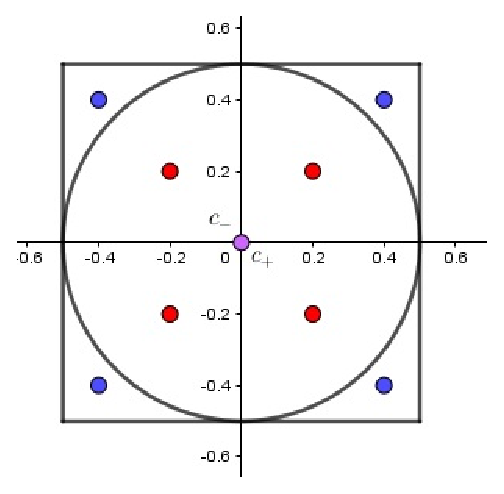
\includegraphics[width=0.5\textwidth]{pi-2d} \centering \caption{Círculo circunscrito no quadrado em 2 dimensões.}
\end{figure}

Dessa maneira, uma alternativa é levar as entradas para três dimensões. Isto será feito projetando o plano 2D sob uma superfície em 3D, especificamente um cone. A equação geral de um cone é dada por: 
\begin{equation}
\left(\frac{x}{a}\right)^{2}+\left(\frac{y}{b}\right)^{2}=\left(\frac{z}{c}\right)^{2}.\label{hiperboloide}
\end{equation}
Neste ponto é necessário prestar atenção em algumas condições que a Mecânica Quântica impõe. Trabalhando com um sistema de 2 qubits, então um estado qualquer do sistema é dado por: 
\begin{equation}
\left|\psi\right\rangle =\sum^{3}_{i=0}a_{i}\left|i\right\rangle .
\end{equation}
Pela condição de normalização, tem-se que $\sum^{3}_{i=0}a^{2}_{i}=1$, o que implica obviamente em que $0\leq a_{i}\leq1$. A princípio, a amplitude $a_{3}$ será ignorada para que seja possível focar nas outras e em um espaço de 3 dimensões. Escrevendo um conjunto de vetores ortogonais no espaço 3D e utilizando as outras três amplitudes: 
\begin{equation}
\begin{split}\left|u\right\rangle  & =\left(a_{0},0,0\right)^{T},\\
\left|v\right\rangle  & =\left(0,a_{1},0\right)^{T},\\
\left|w\right\rangle  & =\left(0,0,a_{2}\right)^{T}.
\end{split}
\end{equation}
Mas, lembrando que, pela condição de normalização, para qualquer vetor escrito como uma combinação linear destes, isto é $\left|b\right\rangle =\left|u\right\rangle +\left|v\right\rangle +\left|w\right\rangle $, não é possível ter módulo maior que $1$, ou seja $\left\Vert \left|b\right\rangle \right\Vert \leq1$. Isso implica no fato de que algumas configurações não são permitidas, por isso é necessário reduzir o tamanho do quadrado inicial, pois neste modelo, seria impossível gerar pontos que correspondessem à algumas coordenadas como por exemplo $\left(x,y\right)=\left(\pm1,\pm1\right)$ . Pode-se notar também que o valor máximo simultâneo de três coeficientes é $1/\sqrt{3}$. Logo, de modo análogo ao que foi feito em duas dimensões, isto é, um quadrado centrado na origem, agora há um cubo de 3 dimensões também centrado na origem, e este cubo está inteiramente contido em uma esfera de raio $1$ o que respeita a condição de normalização, pois é possível apontar para qualquer ponto no interior deste quadrado com um vetor de módulo menor que $1$. Lembrando que até o momento toda discussão centrou-se em $3$ dos coeficientes. Logo, o último coeficiente é responsável por garantir a normalização do vetor de estado do sistema, isto é $a_{3}=\sqrt{1-a^{2}_{0}-a^{2}_{1}-a^{2}_{3}}$ .

Até aqui, foi garantido que as coordenadas $\left(x,y\right)$ assumam valores aceitáveis. Porém, também é necessário garantir que o mesmo também aconteça na coordenada $z$, isto é, é necessário escolher as contantes $a,b,c$ na equação do cone de modo que dado um ponto $\left(x,y\right)$ qualquer, $z$ também esteja contido na caixa, isto é $-1/\sqrt{3}\leq z\leq1/\sqrt{3}.$ Chamando de $f\left(x,y\right)$ a função responsável por projetar o plano 2D nesta superfície, então: 
\begin{equation}
f\left(x,y\right)=z=c\sqrt{\left(\frac{x}{a}\right)^{2}+\left(\frac{y}{b}\right)^{2}}.
\end{equation}
Dito isso, os valores escolhidos foram $\left(a,b,c\right)=\left(\sqrt{2},\sqrt{2},1\right)$ , pois assim é garantido que os pontos mais ``altos'' da superfície ainda estão contidos no cubo, isto é $f\left(\pm\frac{1}{\sqrt{3}},\pm\frac{1}{\sqrt{3}}\right)=\frac{1}{\sqrt{3}}$. Logo: 
\begin{equation}
f\left(x,y\right)=\sqrt{\frac{x^{2}+y^{2}}{2}}.\label{mapa}
\end{equation}
Agora é possível projetar os pontos inicialmente em 2 dimensões em um espaço de 3 dimensões utilizando a função (\ref{mapa}), e, apesar dos pontos médios $\left|c_{\pm}\right\rangle $ estarem aproximadamente nas mesmas coordenadas em $x$ e $y$, deverão apresentar uma distância considerável em $z$, tornando possível a classificação correta de novos pontos.

\begin{figure}[ht]
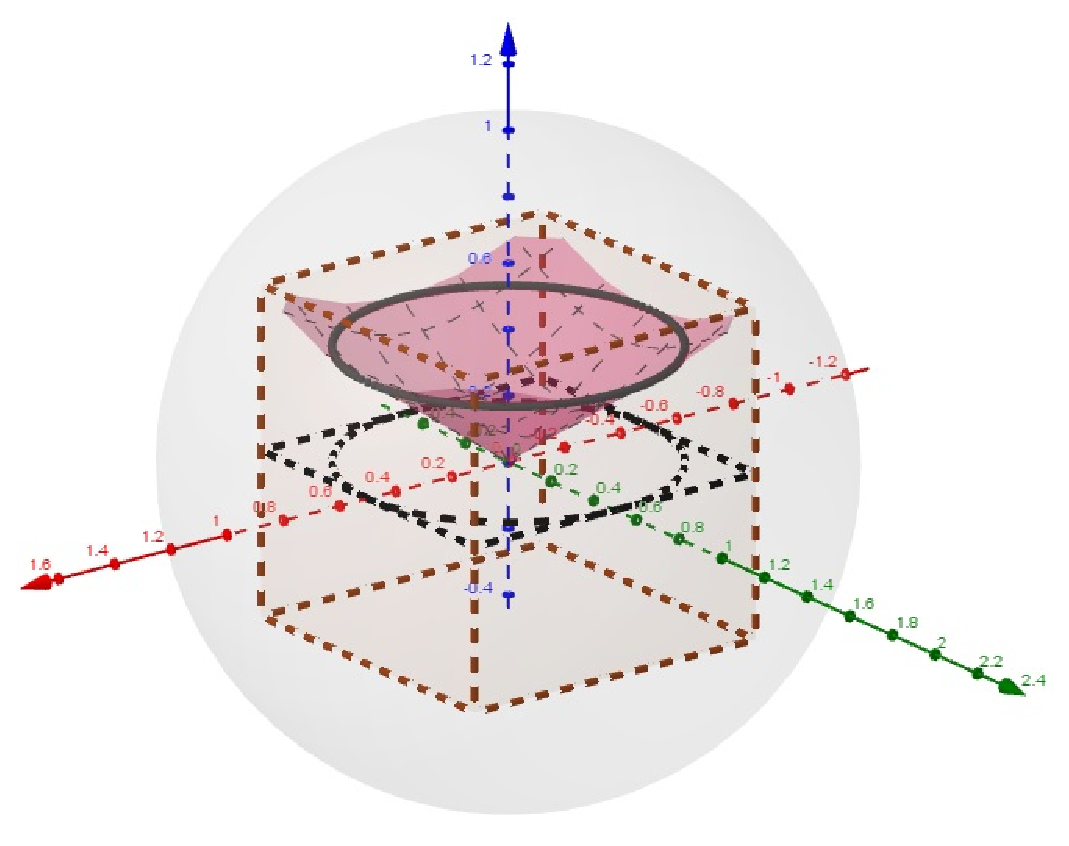
\includegraphics[width=0.75\textwidth]{pi-3d} \centering \caption{Esfera de raio $1$ com o quadrado de lado $1$ em seu interior e a projeção da circunferência no cone.}
\end{figure}

Porém, até agora $a_{3}$ foi negligenciado. Mas o produto interno será calculado em um espaço de 4 dimensões. Pode-se dizer que a última componente da quarta dimensão é inversamente proporcional ao módulo do vetor formado pelas outras 3 componentes. Ainda que não haja recurso visual para visualizar 4 dimensões, o produto interno segue apresentando as propriedades desejas. Por exemplo, dado um vetor $\left|b\right\rangle =\left(b_{0},b_{1},b_{2},\sqrt{1-b^{2}_{0}-b^{2}_{1}-b^{2}_{2}}\right)^{T}$ qualquer, o produto interno dele com ele mesmo apresenta o máximo de semelhança: 
\begin{equation}
\left\langle b|b\right\rangle =b^{2}_{0}+b^{2}_{1}+b^{2}_{2}+1-b^{2}_{0}-b^{2}_{1}-b^{2}_{2}=1.
\end{equation}
Vale destacar duas coisas: apenas a folha de cima do cone é utilizada, e os termos $x$ e $y$ aparecem sempre ao quarado na função (\ref{mapa}), ou seja $z=f\left(\pm x,\pm y\right)$. Então, um vetor em sentido contrário no plano $x\times y$ é $\left|b_{-}\right\rangle =\left(-b_{0},-b_{1},b_{2},\sqrt{1-b^{2}_{0}-b^{2}_{1}-b^{2}_{2}}\right)^{T}$ , e o produto interno então é: 
\begin{equation}
\begin{split}\left\langle b_{-}|b\right\rangle  & =-b^{2}_{0}-b^{2}_{1}+b^{2}_{2}+1-b^{2}_{0}-b^{2}_{1}-b^{2}_{2}\\
 & =2\left(-b^{2}_{0}-b^{2}_{1}\right)+1.
\end{split}
\end{equation}
Os pontos menos semelhantes são pontos nos extremos em que $\left(x,y\right)=\pm\left(0.5,0.5\right)$, então: 
\begin{equation}
\begin{split}\left\langle b_{-}|b\right\rangle  & =2\left(-\frac{1}{4}-\frac{1}{4}\right)+1\\
 & =0.
\end{split}
\end{equation}
Resumindo, nosso método consiste em: 
\begin{itemize}
\item Definimos um quadrado de lado máximo $2/\sqrt{3}$ e centrado na origem; 
\item No interior do quadrado definimos um círculo também centrado na origem; 
\item Geramos pontos aleatórios em 2 dimensões no interior deste quadrado; 
\item Levamos estes pontos para o espaço de \textit{Hilbert} de 4 dimensões, onde cada ponto se torna um vetor do tipo:
\begin{equation}
\left|\psi\right\rangle =a_{0}\left|00\right\rangle +a_{1}\left|01\right\rangle +a_{2}\left|10\right\rangle +a_{3}\left|11\right\rangle .
\end{equation}

\begin{itemize}
\item Sendo os coeficientes dados por: 
\begin{equation}
\begin{split}a_{0} & =x,\\
a_{1} & =y,\\
a_{2} & =\sqrt{\frac{x^{2}+y^{2}}{2}},\\
a_{3} & =\sqrt{1-a^{2}_{0}-a^{2}_{1}-a^{2}_{2}}.
\end{split}
\end{equation}
\end{itemize}
\item Aplicamos então o método kernel no espaço de 4 dimensões e associamos novos pontos à uma das classes binárias (dentro ou fora). 
\end{itemize}
\bibliographystyle{plain}
\bibliography{referencias}

\end{document}
